\begin{theorem}
	Za předpokladu předchozí věty platí
	$$
		\E (s_n^2) = \sigma^2,
	$$
	tedy $s_n^2$ je nestranný odhad $\sigma^2$.
\end{theorem}


\begin{proof}
	$$
		\E(s_n^2)  = \frac{1}{n-2} \E \sum_{i=1}^{n} (Y_i - \hYi)^2 = \frac{1}{n-2} \underbrace{\sumin \E (Y_i - \hYi)^2}_{\text{ozn. } A}
	$$
	
	Protože $\E(\hYi)  = \E(\wbeta_0 + \wbeta_1 x_i) = \beta_0 + \beta_i x_i = \E Y_i$, platí, že:
	$$
	\E(Y_i - \hYi)^2   = \D(Y_i - \hYi) = \E (Y_i - \hYi)^2 - \underbrace{(\E(Y_i - \hYi)^2)}_{= 0}
	$$
	
	Dostáváme tak	
	\begin{align*}
		A & = \sum_{i=1}^{n} \D(Y_i - \hYi) = \sum_{i=1}^n [ \D(Y_i) + \D(\hYi) - 2 \Cov(Y_i, \hYi) ] =  \\
		& = n \sigma^2 + \sum_{i=1}^n \D(\hYi) - 2 \sum_{i=1}^n \Cov(Y_i, \hYi) \tag{$\#$}
	\end{align*}
	
	Rozepíšeme
	$$
		\D \hYi  = \D(\wbeta_o + \wbeta_1 x_i) = \D \wbeta_0 + x_i^2 \D \wbeta_1 + 2 x_i,
	$$
	kde
	$$
		\Cov(\wbeta_0, \wbeta_1) = \Cov(\hYn - \wbeta_1 \hxn, \wbeta_1) = \underbrace{\Cov(\hYn, \wbeta_1)}_{= 0 \text{ (viz. dříve)}} - \hxn \underbrace{\D(\wbeta_1)}_{\frac{\sigma^2}{s_{xx}}} = -\frac{\sigma^2 \hxn}{s_{xx}}
	$$
	a tedy
	\begin{align*}
		\D \hYi & = \sigma^2 \left[ \frac{1}{n} + \frac{\lxn^2}{s_{xx}} + x_i^2 \frac{1}{s_{xx}} - \frac{2 x_i \lxn}{s_{xx}} \right] = \sigma^2 \left[ \frac{1}{n} + \frac{(x_i - \lxn)^2}{s_{xx}}\right] \\
		\sum_{i=1}^n \D \hYi & = \sigma^2 + \frac{\sigma^2}{s_{xx}} \underbrace{\sum_{i=1}^n (x_i - \lxn)^2}_{ = s_{xx}} = 2\sigma^2
	\end{align*}
	
	Následně máme
	\begin{align*}
	\Cov(Y_i, \hYi) & = \Cov(Y_i, \wbeta_0 + \wbeta_1 x_0) = \Cov(Y_i, \wbeta_0) + x_i \Cov(Y_i, \wbeta_1) \\
	\Cov(Y_i, \wbeta_1) & = \frac{1}{s_{xx}} \sum_{j=1}^{n} (x_j - \lxn) \underbrace{\Cov(Y_i, Y_j)}_{= 0 \text{ pro } i \neq j} = \frac{\sigma^2(x_i - \lxn)}{s_{xx}} \\
	\Cov(Y_i, \wbeta_0) & = \Cov(Y_i, \bar{Y}_n - \lxn \wbeta_1) = \Cov(Y_i, \bar{Y}) - \lxn \Cov(Y_i, \wbeta_1) = \frac{\sigma^2}{n} - \frac{\lxn \sigma^2 (x_i - \lxn)}{s_{xx}} \\
	\end{align*}
	a tedy
	\begin{align*}
		\Cov(Y_i, \hYi) & = \frac{\sigma^2}{n} - \frac{\lxn \sigma^2 (x_i - \lxn)}{s_{xx}} + \frac{x_i \sigma^2 (x_i - \lxn)}{s_{xx}} = \frac{\sigma^2}{n} + \frac{\sigma^2}{s_{xx}}(x_i - \lxn)^2 \\
		\sum_{i=1}^n \Cov(Y_i, \hYi) & = \sigma^2 + \frac{\sigma^2}{s_{xx}} \sum_{i=1}^n (x_i - \lxn)^2 = 2 \sigma^2 \\
	\end{align*}
	Dosazením do ($\#$) dostaneme
	$$
		A  = n\sigma^2 + 2\sigma^2 - 4\sigma^2
	$$
	a celkem máme
	$$
		\E(s_n^2)  = \frac{1}{n-2} A = \sigma^2.
	$$
\end{proof}

\begin{corollary}
	Nechť platí předpoklady věty 1 a nechť $e_1, \dots, e_n~iid~\NN(0,\sigma^2)$. Potom platí:
	\begin{enumerate}[a)]
		\item $\frac{(n-2)s_n^2}{\sigma^2} \sim \chi(n-2)$
		\item $s_n^2$ je nezávislé na $\wbeta_0$ a $\wbeta_1$.
	\end{enumerate}
\end{corollary}

\begin{proof}
	Vyplyne z obecnějších tvrzení pro vícerozměrnou regresi.
\end{proof}

\begin{remark}
	Spočetli jsme
	$$
		\underbrace{\D(\wbeta_0)}_{\text{ozn. } \sigma^2(\wbeta_0)} = \sigma^2 \left[ \frac{1}{n} + \frac{\lxn^2}{s_{xx}} \right] \quad \text{a} \quad \underbrace{\D(\wbeta_1)}_{\text{ozn. } \sigma^2(\wbeta_1)} = \frac{\sigma^2}{s_{xx}}
	$$
	
	Nestranné odhady jsou:
	\begin{align*}
		\sigma^2(\wbeta_0) & = s_n^2 \sigma^2 \left[ \frac{1}{n} + \frac{\lxn^2}{s_{xx}} \right] = s_n^2 \delta_0 \\
		\sigma^2(\wbeta_1) & = \frac{s_n^2}{s_{xx}} = s_n^2 \delta_1,
	\end{align*}
	kde $\delta_0$ a $\delta_1$ jsou tzv. variance multiplication factors.
	
	Odhady směrodatné odchylky veličin $\wbeta_0$ a $\wbeta_1$ pak jsou
	$$
		\hat{\sigma}(\wbeta_0) = s_n \sqrt{\delta_0} \quad \text{a} \quad \hat{\sigma}(\wbeta_1) = s_n \sqrt{\delta_1},
	$$
	kterým se pak říká standardní chyby odhadů $\wbeta_0$ a $\wbeta_1$. Hrají zásadní roli při konstrukci IS a TH.
\end{remark}

\section{Gauss - Markov theorem}

\begin{itemize}
	\item Chyby normální $\Rightarrow$ LSE pro $\wbeta_0, \wbeta_1$ je MLE ... parametrů (eficientní odhad)
	\item Pokud nejsou chyby normální, jaké je opodstatnění použít LSE?
	
	Ukážeme, že LSE jsou BLUE (best linear unbiased estimators), tedy lineární nestranné odhady s minimálním rozptylem
	\item Je ale třeba poznamenat, že můžou existovat nelineární nebo vychýlené odhady parametrů $\beta_0, \beta_1$, které jsou eficientnější než LSE, pokud se rozdělení chyb liší výrazně od normálního (tím se zabývá robustní regresní analýza).
\end{itemize}

Uvažujme model
$$
	Y_i = \beta_0 + \beta_1 x_i + e_i, \quad i = 1, \dots, n \text{ (*)}
$$

\begin{define}
	Lineární odhad parametru $\beta$ je statistika tvaru
	$$
		\wbeta = \sumin c_i Y_i,
	$$
	kde $c_i$ jsou dané reálné konstanty a $i = 1, \dots, n$.
\end{define}

\begin{theorem}
	Nechť $e_1, \dots, e_n$ v modelu (*) jsou nekorelované a mají stejný rozptyl $\D(e_i) = \sigma^2, i = 1, \dots, n$. Potom LSE $\wbeta_j, j = 0,1$ je BLUE parametru $\beta_j$.
\end{theorem}

\newcommand{\pd}{\delta}

\begin{proof}
	Ukážeme pro $\beta_1$, pro $\beta_0$ je důkaz podobný.
	
	Nechť $\wbeta_1 = \sumin c_i Y_i$, pak
	
	$\D \wbeta_1 = \sumin c_i^2 \D Y_i = \sigma^2 \sumin c_i^2$
	
	Aby byl $\wbeta_1$ nestranný, musí platit $\E \wbeta_1 = \beta_1$, tedy
	
	$\E \wbeta_1 = \sumin c_i \E Y_i = \beta_0 \sumin c_i + \beta_1 \sumin c_i x_i \overset{!}{=} \beta_1$
	
	protože to musí platit pro lib. $\beta_0, \beta_1$, dostáváme
	$$
		\sumin c_i = 0 \quad \text{a} \quad \sumin c_i x_i = 1.
	$$
	
	Hledání lineárního, nestranného odhadu $\beta_1$ je tedy redukováno na minimalizaci $\sumin c_i^2$ za vazebných podmínek $\sumin c_i = 0 \quad \text{a} \quad \sumin c_i x_i = 1$.
	
	Lagrangeova funkce: $L = \sumin c_i^2 - 2 \lambda_1 (\sumin c_i) - 2 \lambda_2 (\sumin c_i x_i - 1)$.
	
	\begin{gather*}
		\frac{\partial L}{\partial c_i} = 2 c_i - 2 \lambda_1 - 2 \lambda_2 x_i = 0, \quad i = 1, \dots, n \\
		\frac{\partial L}{\partial \lambda_1} = -2 (\sumin c_i) = 0 \\
		\frac{\partial L}{\partial \lambda_2} = -2 (\sumin c_i x_i - 1) = 0
	\end{gather*}
	
	Sečteme prvních $n$ rovnic
	$$
		\underbrace{\sumin c_i}_{= 0} - n \lambda_1 - \lambda_2 \sumin x_i = 0 \Rightarrow n\lambda_1 + \lambda_2 \sumin x_i = 0 \Rightarrow \lambda_1 = - \lambda_2 \lxn
	$$
	
	Sečteme dále prvních $n$ rovnic vynásobených $x_i$:
	\begin{gather*}
		\sumin c_i x_i - \lambda_1 \sumin x_i - \lambda_2 \sumin x_i^2 = 0 \\
		\Rightarrow \lambda_1 \sumin x_i + \lambda_2 \sumin x_i^2 = 1 \\
		 -\lambda_2 \lxn \cdot n \lxn + \lambda_2 \sumin x_i^2 = 1 \\
		 \lambda_2 \left( \sumin x_i^2 - n \lxn^2 \right) = 1 \Rightarrow \lambda_2 = \frac{1}{s_{xx}} \quad \text{a} \quad \lambda_1 = - \frac{\lxn}{s_{xx}}
	\end{gather*}
	
	Dosadíme za $\lambda_1, \lambda_2$:
	$$
		c_i + \frac{\lxn}{s_{xx}} - \frac{x_i}{s_{xx}} = 0 \Rightarrow c_i = \frac{x_i - \lxn}{s_{xx}}
	$$
	a $\wbeta_1 = \frac{1}{s_{xx}} \sumin (x_i - \lxn) Y_i$, což je LSE.

\end{proof}

\begin{remark}
	Ukázali jsme pouze, že to je stacionární bod, že je tam i minimum ukážeme v obecnější větě ve vícerozměrné regresi.
\end{remark}

\section{IS pro $\beta_0, \beta_1$}

\begin{itemize}
	\item IS poskytují jistou "míru přesnosti" bodových odhadů
	\item pro jejich konstrukci potřebujeme znát rozdělení pravděpodobnosti bodového odhadu
	\item budeme tedy uvažovat normalitu chyb
	\item spočtené IS se ale často používají, i když rozdělení chyb není normální, jejich použití se zdůvodňuje tím, že LSE odhady par. $\beta$ jsou lineární funkcí $Y_i, i = 1, \dots, n$, což umožňuje aplikovat CLT a dostat asymptotickou normalitu odhadů $\wbeta_0, \wbeta_1$
\end{itemize}

Uvažujme model $Y_i = \beta_0 + \beta_1 x_i + e_i$, $e_i$ i.i.d $\NN(0,\sigma^2)$. Víme:
$$
	\wbeta_i \sim \NN(\beta_i, \sigma^2(\wbeta_i)), \quad \frac{(n-2)s_n^2}{\sigma^2} \sim \chi^2(n-1) \text{\; a nezávisí na \;} \wbeta_0, \wbeta_1.
$$

\begin{remark}
	$$
		X \sim \NN(0,1), Y \sim \chi^2(n), X, Y \text{ nezávislé } \Rightarrow \frac{X}{\sqrt{Y/n}} \sim t(n)
	$$
\end{remark}

Tedy
$$
	T_i = \frac{\frac{\wbeta_i - \beta_i}{\sigma(\wbeta_i)}}{\frac{s_n}{\sigma}} = \frac{\wbeta_i - \beta_i}{\hat{\sigma}}(\wbeta_i) \sim t(n-2, i = 0,1)
$$
neboť $\sigma(\wbeta_i) = \sigma \sqrt{\delta_i}$ a $\hat{\sigma}(\wbeta_i) = s_n \sqrt{\delta_i}$.

Tzn. $P \left[ -t_{1-\alpha/2}(n-2) \leq \frac{\wbeta_i - \beta_i}{\hat{\sigma}}(\wbeta_i) \leq t_{1-\alpha/2}(n-2) \right]$ a vyjádřením $\beta_i$ dostaneme
$$
	P \left[ \wbeta_i - t_{1-\alpha/2}(n-2) \hat{\sigma}(\wbeta_i) \leq \beta_i \leq  \wbeta_i + t_{1-\alpha/2}(n-2) \hat{\sigma}(\wbeta_i) \right] = 1 - \alpha
$$
a tedy $(\wbeta_i \pm t_{1-\alpha/2}(n-2) \hat{\sigma}(\wbeta_i))$ je $100(1-\alpha)\%$ IS pro $\beta_i, i = 0,1$.

Dosazením za $\hat{\sigma}(\wbeta_i)$ dostaneme

\begin{itemize}
	\item $100(1-\alpha)\%$ IS pro $\beta_0$: $\wbeta_0 \pm t_{1-\alpha/2}(n-2) \cdot s_n \sqrt{\frac{1}{n} + \frac{\lxn^2}{s_{xx}}}$
	\item $100(1-\alpha)\%$ IS pro $\beta_1$: $\wbeta_1 \pm t_{1-\alpha/2}(n-2) \cdot s_n \frac{1}{\sqrt{s_{xx}}}$
\end{itemize}

\begin{remark}
	Z tvarů IS lze pozorovat, že IS pro $\beta_0$ bude ve většině praktických případů širší než IS pro $\beta_1$, tzn. směrnice je obecně odhadnuta s větší přesností než absolutní člen (intercept).
\end{remark}


\begin{remark}
	Někdy se konstruují simultánní IS pro oba parametry. 

\begin{center}
    
    \begin{tikzpicture}
    \node[inner sep=0pt] (pic) at (0,0)
    {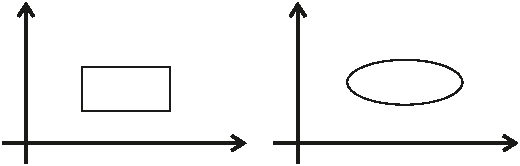
\includegraphics[width=13cm]{pictures/picture_5_M.pdf}};
    \draw [color=black](-6.75,2.4) node[anchor=north west] {$\beta_{0}$};
    \draw [color=black](0,2.4) node[anchor=north west] {$\beta_{0}$};
    \draw [color=black](-1.2,-1.6) node[anchor=north west] {$\beta_{1}$};
    \draw [color=black](5.45,-1.6) node[anchor=north west] {$\beta_{1}$};
    \draw [color=black](2.9,0.25) node[anchor=north west] {$1 - \alpha$};
    \draw [color=black](-3.9,0.2) node[anchor=north west] {$1 - \alpha$};
    \end{tikzpicture}
\end{center}	
	
	 Zmíníme podrobněji u vícerozměrné regrese.
\end{remark}


\subsection{TH pro $\beta_0, \beta_1$}

Chtěli bychom ověřit platnost předpokladu lineárního vztahu mezi $x$ a $y$.

Předpokládejme nyní, že model je lineární a že $x$ je jediná dostupná vysvětlující proměnná. Otázoku je, zda je $x$ užitečná ve vysvětlení variability v $y$, chceme tedy rozhodnout mezi dvěma modely:
$$
	Y_i = \beta_0 + e_i \quad \text{a} \quad Y_i = \beta_0 + \beta_1 x_i + e_i
$$
tzn. otestovat hypotézu $\hypothesis{\beta_1 = 0}{}\beta_1 \neq 0$.

Pokud nezamítneme $H_0$, závěr bude, že $x$ nevysvětluje nic z variability $y$ a není v modelu významné. Pokud zamítneme $H_0$, znamená to, že $x$ je významné.

\begin{remark}
	Tyto závěry jsou správné pouze za předpokladu, že model je lineární!
	\begin{itemize}
		\item nezamítnutí $H_0$ nemusí znamenat, že $x$ není užitečná, může to pouze indikovat, že vztah mezi $y$ a $x$ není lineární
		\item zamítnutí $H_0$ naopak ří, že existuje lineární trend mezi $x$ a $y$, ale mohou tam být i jiné typy závislosti
	\end{itemize}
\end{remark}

Pro konstrukci testů využijeme odvozené IS.

\begin{remark}
	Opakování: $\hypothesis{\theta = \theta_0}{\theta \neq \theta_0} \Rightarrow (\underline{\theta}, \bar{\theta})$ je $100(1-\alpha)\%$ IS pro $\theta$. Pak $W = \{ x | \theta_0 \notin (\underline{\theta}, \bar{\theta}) \}$ je kritický obor test na hladině $\alpha$.
\end{remark}

$H_0: \beta_1 = 0$ zamítneme, pokud $0 \notin \left( \wbeta_1 \pm t_{1-\alpha/2}(n-2) \cdot  \frac{s_n}{\sqrt{s_{xx}}} \right)$, tzn.
\begin{gather*}
	\text{buď } \wbeta_1 + t_{1-\alpha/2}(n-2) \cdot  \frac{s_n}{\sqrt{s_{xx}}} < 0 \iff  \wbeta_1 \frac{\sqrt{s_{xx}}}{s_n} < - t_{1-\alpha/2}(n-2) \\
	\text{nebo } \wbeta_1 - t_{1-\alpha/2}(n-2) \cdot  \frac{s_n}{\sqrt{s_{xx}}} > 0 \iff \wbeta_1 \frac{\sqrt{s_{xx}}}{s_n} > t_{1-\alpha/2}(n-2)
\end{gather*}
A zapsáno dohromady
$$
	|T_n| = |\wbeta_1| \frac{\sqrt{s_{xx}}}{s_n} > t_{1-\alpha/2}(n-2).
$$

\begin{remark}
	Intuitivní interpretace: $|T_n| = |\wbeta_1| \frac{\sqrt{s_{xx}}}{s_n} = \frac{|\wbeta_1|}{\hat{\sigma}(\wbeta_1)}$ je převrácená hodnota relativní chyby.
	
	Pokud je $\beta_1$ dobře odhadnuto, očekáváme malý rozptyl $\hat{\sigma}(\wbeta_1)$, tedy $T$ bude velké.
	
	t-test tedy říká, že zamítneme $H_0$, pokud je relativní chyba odhadu malá.
\end{remark}